\documentclass[conference]{IEEEtran}

\usepackage{cite}
\usepackage{amsmath,amssymb,amsfonts}
\usepackage{graphicx}
\usepackage{textcomp}
\usepackage{xcolor}
\usepackage{booktabs}
\usepackage{array}
\usepackage[hidelinks]{hyperref}
\usepackage{balance}
\usepackage{tikz}
\usetikzlibrary{arrows.meta}

\hypersetup{
  pdfauthor={Anonymous},
  pdftitle={Layered Instruction Fine Tuning Cyber Threat Intelligence for Small Language Models: A Functional Approach},
  pdfsubject={Double-blind conference submission},
  pdfkeywords={small language models, cyber threat intelligence, vulnerability management, layered instruction fine-tuning, knowledge graphs, data provenance}
}

\begin{document}
\bstctlcite{BSTcontrol}

\title{Layered Instruction Fine Tuning Cyber Threat Intelligence for Small Language Models: A Functional Approach}

\author{\IEEEauthorblockN{Anonymous Authors}}

\maketitle
\pagestyle{plain}
\thispagestyle{plain}

\begin{abstract}
Vulnerability response in security operations is a chain of mapping decisions: a newly disclosed CVE must be scored for severity and exploitability, traced to its weakness class and the adversary techniques it enables, and linked to mitigations and detections before a patch or compensating control is scheduled. Because the asset and exposure context behind these decisions often cannot leave the organization, locally served small language models (SLMs) are attractive, but only if their outputs land on the correct catalog identifier and their training targets are traceable to source intelligence. We present an SLM specialization workflow built on a versioned Neo4j graph joining twelve public threat and vulnerability intelligence sources (e.g., NVD, CISA KEV, EPSS, CWE, ATT\&CK) (\emph{Ariadne}), and a template engine that materializes each instruction target by executing a typed graph query (\emph{Sophia}). Using a functionally optimized approach, we use a layered Instruction Fine-Tuning (IFT) template-based strategy to train Qwen2.5-32B-Instruct by which we increase attack-technique extraction scores from 18.2 to 65.8, vulnerability mitigation selection scores from 7.6 to 62.5, and the three-benchmark mean we use for testing from 57.7 to 65.0 (95\% bootstrap interval 64.1--66.0), with an 11.6-point decrease on the MMLU-Pro general-knowledge benchmark.
\end{abstract}

\begin{IEEEkeywords}
small language models, SLMs, cyber threat intelligence, CTI, vulnerability management, cyber security, instruction fine-tuning, IFT, knowledge graphs, data provenance
\end{IEEEkeywords}

\section{Introduction}
For each newly disclosed CVE~\cite{cve} found in a vulnerability scan of a given environment, security analysts must join intelligence from separate, largely public catalogs: the NVD CVSS vector~\cite{nvd}, exploitation likelihood from EPSS~\cite{jacobs2021epss}, confirmed exploitation from the CISA Known Exploited Vulnerabilities (KEV) catalog~\cite{cisakev}, public exploit code~\cite{exploitdb,pocingithub}, the CWE weakness~\cite{cwe} and CAPEC attack patterns~\cite{capec} behind the flaw, the ATT\&CK techniques it enables~\cite{strom2018attack}, and the related mitigations, D3FEND countermeasures~\cite{d3fend}, and Sigma detections~\cite{sigma}. This analysis must then be combined with sensitive local context (asset inventory, scanner findings, exposure, business criticality) to plan the optimal risk response (patch now, apply a compensating control, or add detection until a maintenance window), a per-vulnerability analysis that NIST notes organizations lack the time and expertise to perform manually~\cite{nist80040r4}.

Each join maps free text into a controlled vocabulary, and near-misses are costly: a parent ATT\&CK technique in place of the sub-technique points detection engineering at the wrong telemetry; a related but incorrect CWE suggests the wrong compensating control; a wrong CVSS Attack Vector moves a vulnerability between remediation tiers; a misnormalized threat actor misdirects hunting; and an unparseable answer breaks downstream ticketing and orchestration. CTIBench~\cite{ctibench} and a public benchmark anonymized here as \emph{Benchmark A}~\cite{anonbench} test models on exactly these mappings (Section~\ref{sec:eval}).

That private context, which may include regulated data such as PHI and PII, along with licensed intelligence under sharing restrictions, is exactly what contractual, confidentiality, and data-residency obligations keep away from hosted LLM APIs, frontier models included, favoring locally served open-weight models. We use \emph{small language model} (SLM) operationally for such locally specialized models, not as a parameter threshold: the primary base model has 32B parameters, and we also test 8B, 14B, and sparse 30B-class bases.

The standard way to specialize such a model is \emph{instruction fine-tuning} (IFT): continued supervised training on (instruction, input, output) \emph{triples}, so that the model learns to produce the output when given the instruction and input. Applying IFT to CTI raises two problems. First, the outputs must be correct and traceable: a recommendation that justifies an emergency change or a patch exception must lead back to a source record, yet triples synthesized by another language model are hard to trace to any source fact. Second, a model fine-tuned for several analyst tasks can lose one capability while gaining another, and a single final score hides such losses.

We address the first problem with two components. \emph{Ariadne} is a versioned Neo4j knowledge graph that merges the twelve public sources above into one typed schema. \emph{Sophia} generates IFT triples from expert-written templates: each template compiles to a graph query, and its placeholders are filled from the query's results, so every training target is derived from specific graph records rather than written by a language model. Private entities such as assets and scanner findings fit the same schema but are not used here. We address the second problem with \emph{layered IFT}: rather than one pass over a mixed corpus, the model is fine-tuned in four successive layers (catalog mapping, threat-actor attribution, SOC-style structured response, and recalibration), each starting from the previous layer's checkpoint, and every intermediate checkpoint is retained and evaluated.

Our contributions are: (i)~a graph-grounded data pipeline that produced a 219,675-row core training corpus in which every row resolves to its template, graph binding, and public source identifiers; (ii)~a layered IFT recipe that, applied to Qwen2.5-32B-Instruct, raises attack-technique extraction from 18.2 to 65.8, mitigation selection from 7.6 to 62.5, CTI knowledge from 52.9 to 75.5, and CVE-to-CWE mapping from 59.5 to 67.1, lifting the three-benchmark mean from 57.7 to 65.0 (95\% interval 64.1--66.0), within 1.0 point of DeepSeek-V3.2-Exp and 1.6 points above Gemini-2.5-Flash, at a cost of 11.6 points on MMLU-Pro; (iii)~a checkpoint-level diagnosis of interference: the attribution layer raises canonical threat-actor attribution by 18.4 points, while the SOC-oriented layer raises CyberSOCEval malware accuracy by 19.7 points but erases 33.5 points of canonical attribution; and (iv)~an overlap audit showing that test items whose exact gold fact appears in training score no higher than items whose fact is absent (e.g., 66.4 vs.\ 64.3 on CVE-to-CWE mapping). Code is cited through an anonymized artifact~\cite{anonartifact}.

Section~\ref{sec:related} reviews related work; Sections~\ref{sec:data} and~\ref{sec:layered} present the data pipeline and the layered IFT recipe; Sections~\ref{sec:eval}--\ref{sec:results} cover evaluation, the overlap audit, and results; and Section~\ref{sec:discussion} discusses implications and limitations.

\section{Related Work}\label{sec:related}
\subsection{Instruction Fine-Tuning and Sequential Specialization}
IFT adapts a pretrained language model by continuing training on examples that pair a task instruction, and optionally an input, with the desired response; the loss is computed on the response tokens, so the model learns to produce the response given the instruction. FLAN showed that IFT on many instruction-formulated tasks transfers to unseen tasks~\cite{wei2022flan}; InstructGPT combined supervised demonstrations with preference-based training~\cite{ouyang2022training}; and later work studied how IFT scales with the number and mixture of tasks~\cite{chung2024scaling}. Continued training on domain text further improves domain tasks, motivating a separation between broad domain absorption and narrow task behavior~\cite{gururangan2020dont}. Fine-tuning one model sequentially on several datasets, however, exposes it to \emph{catastrophic interference}: learning a later task can overwrite behavior acquired earlier~\cite{mccloskey1989catastrophic}. Layered IFT is a sequential schedule designed to make this interference observable rather than to eliminate it.

\subsection{Security Instruction Tuning}
CyberPal.AI's SecKnowledge pipeline combines expert-defined schemas, structure-driven generation, BRON graph paths, and LLM-augmented content generation~\cite{levi2025cyberpal}; follow-on work develops cybersecurity-expert SLMs with an enriched instruction pipeline using expert steering and LLM-driven multi-step grounding~\cite{levi2025slm}. SEvenLLM builds a bilingual CTI instruction corpus and benchmark~\cite{ji2024sevenllm}, and CyberBench pairs a multi-task cybersecurity benchmark with instruction-tuned CyberInstruct models~\cite{liu2024cyberbench}. These systems motivate domain-specific supervision, but none makes every training label the deterministic result of an executed graph query (Table~\ref{tab:related}).

\begin{table*}[t]
\caption{Positioning against closely related security instruction-tuning systems. ``Partial'' indicates structured schemas, graph paths, or grounding traces for portions of the pipeline without making every generated label the deterministic result of an executed typed graph query.}
\label{tab:related}
\centering
\scriptsize
\setlength{\tabcolsep}{3pt}
\begin{tabular}{@{}p{0.15\textwidth}p{0.19\textwidth}p{0.19\textwidth}p{0.17\textwidth}p{0.20\textwidth}@{}}
\toprule
System & Graph-grounded targets & LLM-generated training text & Retained layer checkpoints & Provenance of a training label \\
\midrule
CyberPal.AI / SecKnowledge~\cite{levi2025cyberpal} & Partial: expert schemas and BRON graph paths for subsets & Yes: content-grounded LLM augmentation & Multi-phase data generation; retained training-stage checkpoint analysis not reported & Structured source/schema traces; some path explanations are LLM-generated \\
Cybersecurity-expert SLMs~\cite{levi2025slm} & Partial: LLM-driven multi-step grounding & Yes: enriched reasoning traces & Data-enrichment and fine-tuning pipeline; layer effects not isolated & Enriched traces with expert-in-the-loop steering \\
This work & Yes: typed Ariadne queries materialize every Sophia CTI row & No for Sophia targets; auxiliary general mixtures are external & Yes: Core, +TAA, CSE, and recalibration checkpoints retained and evaluated & Row resolves to template, graph binding, and public-source keys \\
\bottomrule
\end{tabular}
\end{table*}

\subsection{CTI Knowledge Graphs}
Open-CyKG constructs an open cyber-threat knowledge graph from unstructured reports~\cite{sarhan2021opencykg}. That work concerns how facts enter a graph; this work concerns how a populated graph is turned into IFT triples. The two qualities should not be conflated: a Sophia target is traceable to its graph binding, but the graph can still contain incomplete, stale, or misinterpreted source facts.

\section{Graph-Grounded Training Data}\label{sec:data}
\subsection{Formulation}
An IFT triple $r=(i,x,y)$ consists of an instruction $i$, an optional input or question $x$, and a target output $y$. Let $G_t=(V_t,E_t,A_t)$ be the Ariadne graph at snapshot $t$, with typed nodes $V_t$, typed relationships $E_t$, and node attributes $A_t$. A Sophia template $\tau$ is text with typed placeholders in its instruction, question, and answer parts $(i_\tau,x_\tau,y_\tau)$; it compiles to a graph query $q_\tau$ that includes any constraints the template declares. Executing the query returns a set of bindings $q_\tau(G_t)$, each binding $b$ assigning a node, relationship, or attribute value to every placeholder. For each binding $b\in q_\tau(G_t)$, Sophia emits one triple
\begin{equation}
 r_{\tau,b}=\big(\operatorname{render}(i_\tau,b),\,\operatorname{render}(x_\tau,b),\,\operatorname{render}(y_\tau,b)\big),
\end{equation}
where $\operatorname{render}(s,b)$ replaces each placeholder in text $s$ with its value under $b$. In short, a template generates one IFT triple per query result. Each row also records its template identifier and source tags, linking it to the template, snapshot, and public identifiers it was built from.

The fine-tuned model $p_\theta(y\mid i,x)$ is trained with the standard next-token cross-entropy on the target tokens. For layer $s$ with dataset $D_s$,
\begin{equation}
 \mathcal{L}_s(\theta)=-\sum_{(i,x,y)\in D_s}\sum_{j=1}^{|y|}\log p_\theta(y_j\mid i,x,y_{<j}),
\end{equation}
with the checkpoint from layer $s-1$ initializing layer $s$. No new optimizer, loss, or architecture is introduced; the method lies in how each $D_s$ is generated and in how the layers are sequenced.

\subsection{Ariadne: Graph Schema}
Ariadne is a Neo4j property graph built from the twelve public sources in Table~\ref{tab:schema}, grouped into seven layers. Each source contributes typed nodes keyed by their natural identifiers (STIX, CVE, CWE, CAPEC, or D3FEND IDs). Ingestion uses Neo4j \texttt{MERGE} operations under uniqueness constraints on those keys, so re-running it never duplicates nodes, and it follows dependency order---framework catalogs, then vulnerabilities, then exploit evidence---so every cross-framework relationship has both endpoints present. The relationships most used by templates form a spine from vulnerability to weakness to attack pattern to adversary technique, with mitigations, countermeasures, and detections attached to techniques and exploitation signals attached to vulnerabilities. The snapshot used here holds about 280,000 nodes and 480,000 relationships. Bounded catalogs are loaded in full; the high-churn vulnerability and exploit feeds are scoped to 2024 onward. EPSS and the current-year NVD feed are refreshed daily and other sources on explicit refresh, so dataset freshness is tracked per source.

\begin{table}[t]
\caption{Ariadne layers, sources, principal entity types, and the main cross-framework links that templates traverse.}
\label{tab:schema}
\centering
\scriptsize
\setlength{\tabcolsep}{2.5pt}
\begin{tabular}{@{}p{0.18\columnwidth}p{0.21\columnwidth}p{0.27\columnwidth}p{0.26\columnwidth}@{}}
\toprule
Layer & Sources & Principal entities & Main links \\
\midrule
Adversary behavior & ATT\&CK, Engage & techniques, groups, software, mitigations; engagement activities & technique--mitigation; technique--group \\
Weakness \& attack pattern & CWE, CAPEC & weaknesses; attack patterns & CAPEC$\rightarrow$CWE; CAPEC$\rightarrow$technique \\
Vulnerability & CVE, NVD & CVE records; CVSS vectors; affected products & CVE$\rightarrow$CWE; CVE$\rightarrow$CAPEC \\
Exploitation signal & CISA KEV, EPSS & KEV entries; exploitation probabilities & $\rightarrow$CVE \\
Exploit evidence & ExploitDB, PoC-in-GitHub & exploit and proof-of-concept records & $\rightarrow$CVE \\
Counter\-measure & D3FEND & defensive techniques & D3FEND--technique \\
Detection & Sigma & detection rules & rule$\rightarrow$technique \\
\bottomrule
\end{tabular}
\end{table}

\subsection{Sophia: Template-Driven Triple Generation}
A Sophia template is plain text with placeholders in braces. A placeholder \texttt{\{a:Label.prop\}} binds alias \texttt{a} to a node of type \texttt{Label} and inserts its property \texttt{prop}; \texttt{\{a.rel>Label.prop\}} follows relationship \texttt{rel} from the node bound to \texttt{a}; and \texttt{\{a.prop\}} reuses an existing binding. Hidden sections \texttt{<*\{\ldots\}*>} add bindings or constraints to the query without producing text. The language also supports any/all filters over list-valued properties, list expansion, and source prefixes that distinguish same-named types such as ATT\&CK and CAPEC attack patterns. A simple template binds one ATT\&CK technique and emits its properties:
\begin{quote}\scriptsize\ttfamily\sloppy
Question: Explain ATT\&CK technique \{ap:attack-pattern.name\} (\{ap.id\}) and how it is used.\\
Answer: Technique \{ap.name\} (\{ap.id\}) is described as: \{ap.description\}. Commonly observed across \{ap.x\_mitre\_platforms\}.
\end{quote}
Executed against Ariadne, this template yields one triple per technique node. Templates become more useful when they traverse relationships across frameworks. The following template from the generator's library correlates a CVE with its attack pattern and weakness:
\begin{quote}\scriptsize\ttfamily\sloppy
Instruction: You are a cybersecurity expert that has been trained to give precise responses to complex cybersecurity questions. You work in a SOC protecting data for enterprise customers helping to protect their digital assets.\\
Question: Correlate CVE, CWE, and CAPEC for a single vulnerability chain.\\
Answer: CVE \{cve:CVE.id\} impacts CAPEC \{cap:cve.impacts>CAPEC.name\} and is categorized as weakness \{cwe:cve.problemType>Weakness.name\}. CAPEC \{cap.id\} exploits weakness \{cwe2:cap.exploits>Weakness.name\}. <*\{force cwe.id=cwe2.id\}*>
\end{quote}
The template compiler turns each binding into a \texttt{MATCH} pattern of a Cypher query and the hidden \texttt{force} section into a \texttt{WHERE} condition, schematically:
\begin{quote}\scriptsize\ttfamily
MATCH (cve:CVE)-[:impacts]->(cap:CAPEC),\\
\hspace*{1em}(cve)-[:problemType]->(cwe:Weakness),\\
\hspace*{1em}(cap)-[:exploits]->(cwe2:Weakness)\\
WHERE cwe.id = cwe2.id RETURN cve, cap, cwe, cwe2
\end{quote}
Only chains in which the CVE's own weakness is also the weakness the attack pattern exploits are returned, and each returned row is rendered into one triple whose answer names the CVE, the attack pattern, and the weakness. Any generated answer can therefore be checked by re-running its query. Negative examples use inequality constraints; because CTI graphs are incomplete, such examples mean ``not supported by the graph'' rather than ``false in the world.''

Generation runs in three steps: templates are extracted from their authoring documents; each is executed against Ariadne, producing its triples and a report of failed or empty queries; and the results are merged into one dataset. Rows are then balanced across template families, deduplicated, screened for overlap with evaluation data (Section~\ref{sec:overlap}), license-gated, and serialized as JSON. Schema tests catch templates that reference absent node types, relationships, or properties, but they do not replace expert review of whether a template's mapping is semantically right: Sophia guarantees a deterministic path from query to target, not the correctness of every upstream fact.

\begin{figure*}[t]
    \centering
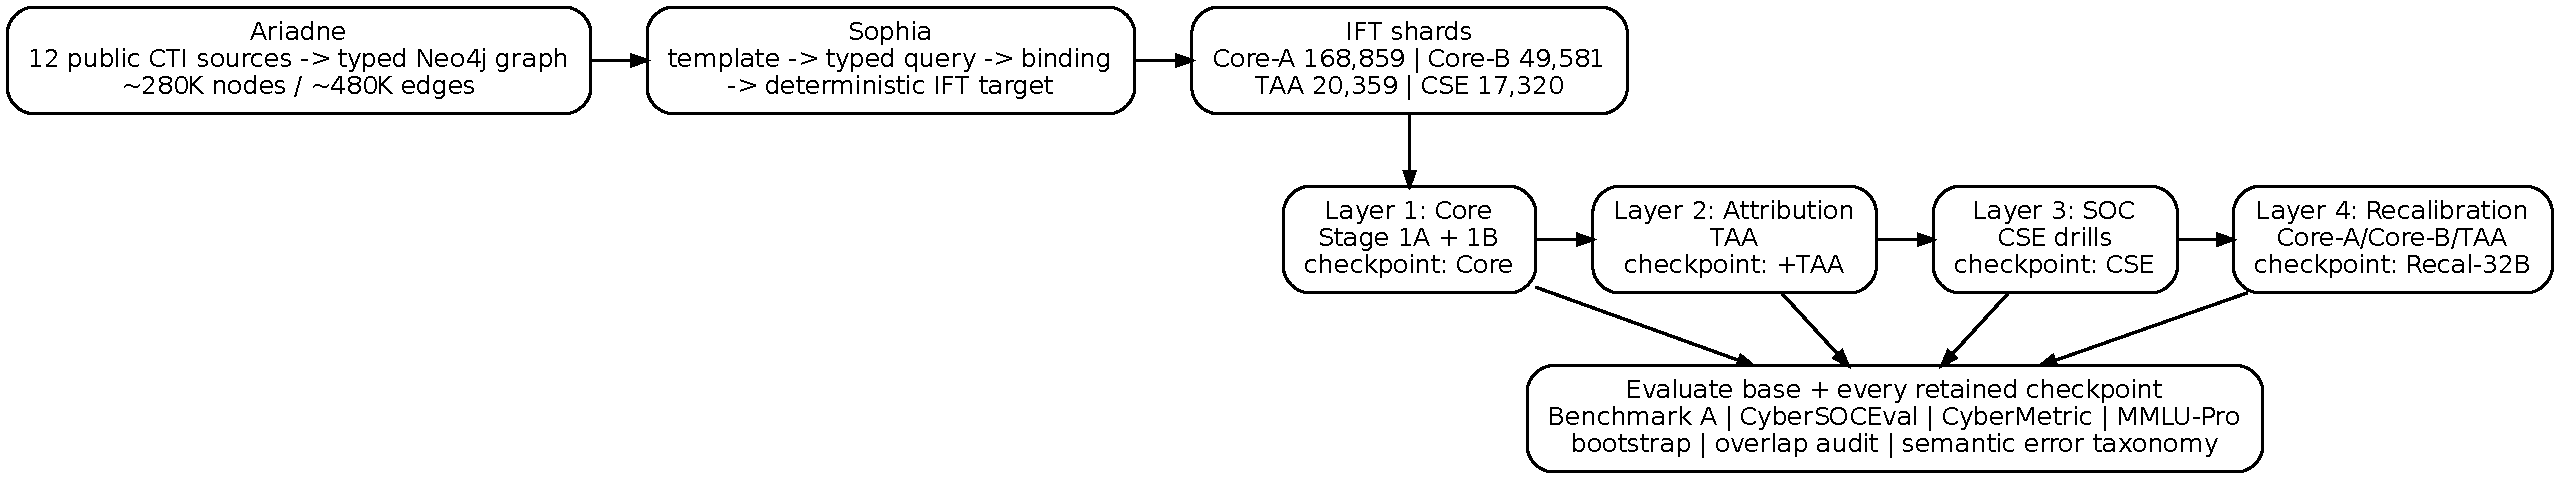
\includegraphics[width=0.98\textwidth]{figures/pipeline_greek_blind.pdf}
    \caption{Data and training pipeline. Ariadne integrates twelve public CTI sources into a versioned typed graph; Sophia executes template queries against it and renders one IFT triple per result; the resulting shards feed four IFT layers whose checkpoints are all retained and evaluated.}
    \label{fig:pipeline}
\end{figure*}

\subsection{Training Corpus}
A \emph{shard} is the set of triples generated for one training layer. The build produced four training shards and three validation shards, the latter holding out 50 rows per template family. The core corpus contained 219,675 rows after balancing; after the overlap screen removed 684 rows and 550 were held out for validation, it was split into Core-A (168,859 rows: knowledge, multiple-choice, mitigation, attribution, and SOC families) and Core-B (49,581 rows: drills for the RMS, ATE, VSP, and RCM tasks of Table~\ref{tab:eval}). The TAA (attribution) and CSE (SOC-style response) shards contain 20,359 and 17,320 rows. Core-A is mixed with general-purpose instruction data from the T\"ulu-3 SFT~\cite{lambert2024tulu} and Stanford Alpaca~\cite{taori2023alpaca} datasets to limit loss of general ability; these auxiliary examples are not generated by Sophia.

\section{Layered Instruction Fine-Tuning}\label{sec:layered}
Layered IFT trains the model in successive layers, each a separate supervised run on its own shard that starts from the previous layer's checkpoint. Fig.~\ref{fig:layered} summarizes the data, functional areas, quantities, and settings of each layer, and what each retained checkpoint gained or lost. Each layer targets one analyst role, and its checkpoint is retained so that both its gains and any damage to earlier skills can be measured. Checkpoints are named after their layer: Core, +TAA, CSE, and Recal-32B, the final 32B checkpoint.

\begin{figure*}[t]
\centering
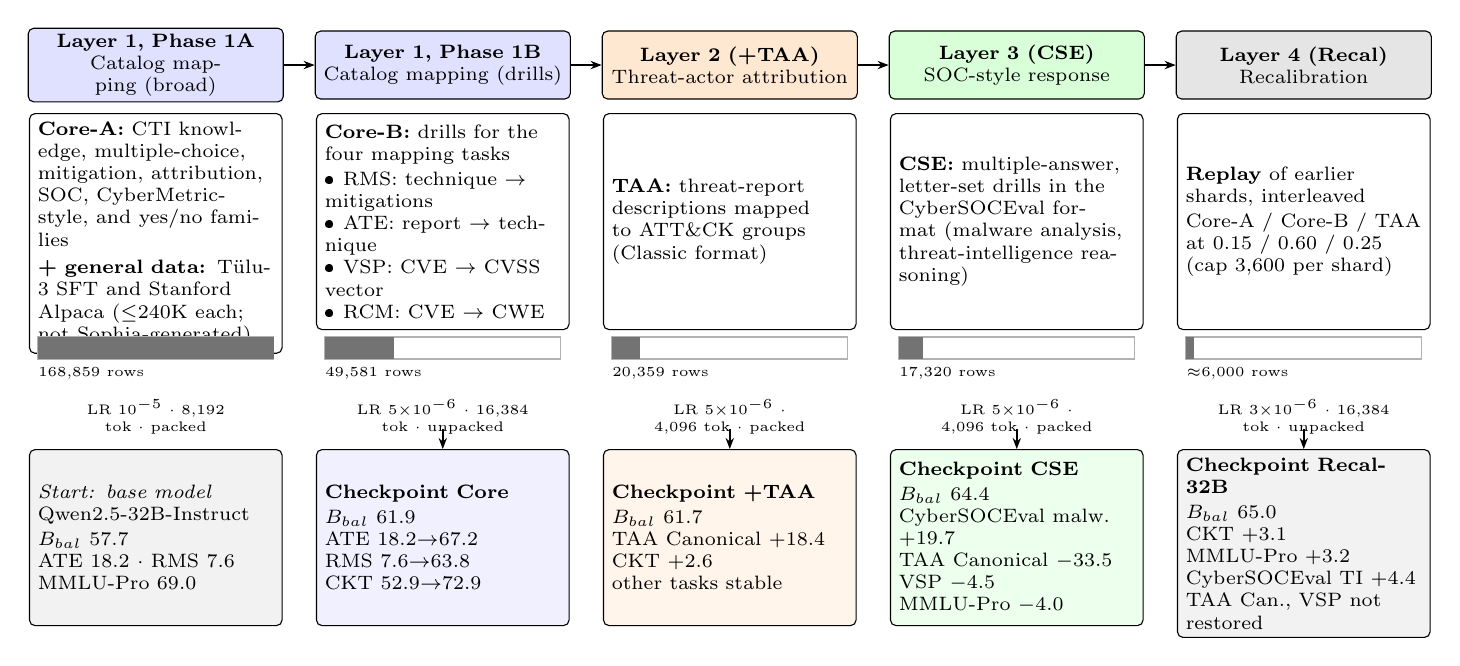
\begin{tikzpicture}[
  x=1in, y=1in, font=\scriptsize,
  hdr/.style={draw, rounded corners=2pt, fill=#1, align=center, text width=1.22in, minimum height=0.34in, inner sep=2pt},
  dat/.style={draw, rounded corners=2pt, fill=white, align=left, text width=1.18in, minimum height=1.08in, inner sep=3pt, anchor=north},
  ckp/.style={draw, rounded corners=2pt, fill=#1, align=left, text width=1.18in, minimum height=0.88in, inner sep=3pt, anchor=north},
  arr/.style={-{Stealth[length=4pt]}, semithick},
  bar/.style={fill=black!55, draw=none}
]
\def\W{1.30}\def\G{0.135}
% column centres
\foreach \i in {0,...,4} { \pgfmathsetmacro{\x}{\i*(\W+\G)+\W/2} \expandafter\xdef\csname cx\i\endcsname{\x} }
% ---------- headers
\node[hdr=blue!12]   (h0) at (\csname cx0\endcsname,0) {\textbf{Layer 1, Phase 1A}\\Catalog mapping (broad)};
\node[hdr=blue!12]   (h1) at (\csname cx1\endcsname,0) {\textbf{Layer 1, Phase 1B}\\Catalog mapping (drills)};
\node[hdr=orange!18] (h2) at (\csname cx2\endcsname,0) {\textbf{Layer 2 (+TAA)}\\Threat-actor attribution};
\node[hdr=green!15]  (h3) at (\csname cx3\endcsname,0) {\textbf{Layer 3 (CSE)}\\SOC-style response};
\node[hdr=black!10]  (h4) at (\csname cx4\endcsname,0) {\textbf{Layer 4 (Recal)}\\Recalibration};
\foreach \a/\b in {h0/h1,h1/h2,h2/h3,h3/h4} \draw[arr] (\a) -- (\b);
% ---------- training data
\node[dat] (d0) at (\csname cx0\endcsname,-0.24) {\textbf{Core-A:} CTI knowledge, multiple-choice, mitigation, attribution, SOC, CyberMetric-style, and yes/no families\\[2pt]\textbf{+ general data:} T\"ulu-3 SFT and Stanford Alpaca ($\le$240K each; not Sophia-generated)};
\node[dat] (d1) at (\csname cx1\endcsname,-0.24) {\textbf{Core-B:} drills for the four mapping tasks\\[1pt]
\textbullet\ RMS: technique $\rightarrow$ mitigations\\
\textbullet\ ATE: report $\rightarrow$ technique\\
\textbullet\ VSP: CVE $\rightarrow$ CVSS vector\\
\textbullet\ RCM: CVE $\rightarrow$ CWE};
\node[dat] (d2) at (\csname cx2\endcsname,-0.24) {\textbf{TAA:} threat-report descriptions mapped to ATT\&CK groups (Classic format)};
\node[dat] (d3) at (\csname cx3\endcsname,-0.24) {\textbf{CSE:} multiple-answer, letter-set drills in the CyberSOCEval format (malware analysis, threat-intelligence reasoning)};
\node[dat] (d4) at (\csname cx4\endcsname,-0.24) {\textbf{Replay} of earlier shards, interleaved\\[1pt]
Core-A / Core-B / TAA\\ at 0.15 / 0.60 / 0.25\\ (cap 3,600 per shard)};
% ---------- row-count bars (linear scale, full width = 168,859 rows)
\def\BW{1.18}
\foreach \i/\n/\lab in {0/168.859/{168,859 rows},1/49.581/{49,581 rows},2/20.359/{20,359 rows},3/17.320/{17,320 rows},4/6.000/{$\approx$6,000 rows}} {
  \pgfmathsetmacro{\xl}{\csname cx\i\endcsname-\BW/2}
  \pgfmathsetmacro{\bl}{\n/168.859*\BW}
  \draw[black!30] (\xl,-1.47) rectangle ++(\BW,0.11);
  \fill[bar] (\xl,-1.47) rectangle ++(\bl,0.11);
  \node[anchor=north west, inner sep=0pt, font=\tiny] at (\xl,-1.51) {\lab};
}
% ---------- settings
\foreach \i/\s in {0/{LR $10^{-5}$ $\cdot$ 8,192 tok $\cdot$ packed},1/{LR $5{\times}10^{-6}$ $\cdot$ 16,384 tok $\cdot$ unpacked},2/{LR $5{\times}10^{-6}$ $\cdot$ 4,096 tok $\cdot$ packed},3/{LR $5{\times}10^{-6}$ $\cdot$ 4,096 tok $\cdot$ packed},4/{LR $3{\times}10^{-6}$ $\cdot$ 16,384 tok $\cdot$ unpacked}}
  \node[anchor=north, font=\tiny, text width=1.22in, align=center, inner sep=0pt] at (\csname cx\i\endcsname,-1.67) {\s};
% ---------- checkpoints
\node[ckp=black!5] (c0) at (\csname cx0\endcsname,-1.92) {\textit{Start: base model}\\Qwen2.5-32B-Instruct\\[1pt]$B_{bal}$ 57.7\\ATE 18.2 $\cdot$ RMS 7.6\\MMLU-Pro 69.0};
\node[ckp=blue!6] (c1) at (\csname cx1\endcsname,-1.92) {\textbf{Checkpoint Core}\\[1pt]$B_{bal}$ 61.9\\ATE 18.2$\rightarrow$67.2\\RMS 7.6$\rightarrow$63.8\\CKT 52.9$\rightarrow$72.9};
\node[ckp=orange!8] (c2) at (\csname cx2\endcsname,-1.92) {\textbf{Checkpoint +TAA}\\[1pt]$B_{bal}$ 61.7\\TAA Canonical +18.4\\CKT +2.6\\other tasks stable};
\node[ckp=green!7] (c3) at (\csname cx3\endcsname,-1.92) {\textbf{Checkpoint CSE}\\[1pt]$B_{bal}$ 64.4\\CyberSOCEval malw. +19.7\\TAA Canonical $-$33.5\\VSP $-$4.5\\MMLU-Pro $-$4.0};
\node[ckp=black!5] (c4) at (\csname cx4\endcsname,-1.92) {\textbf{Checkpoint Recal-32B}\\[1pt]$B_{bal}$ 65.0\\CKT +3.1\\MMLU-Pro +3.2\\CyberSOCEval TI +4.4\\TAA Can., VSP not restored};
\foreach \i in {1,...,4} \draw[arr] (\csname cx\i\endcsname,-1.82) -- (c\i.north);
\end{tikzpicture}
\caption{Layered IFT of Qwen2.5-32B-Instruct. Each layer is a separate supervised run on its own shard (row: training data and functional areas; bar: realized training rows on a common linear scale; then learning rate, maximum sequence length, and packing) that starts from the previous layer's weights. Phases 1A and 1B run back to back and only the merged Core checkpoint is retained. Checkpoint boxes give $B_{bal}$ and the most notable changes; changes for +TAA, CSE, and Recal-32B are relative to the preceding checkpoint (Table~\ref{tab:transitions}).}
\label{fig:layered}
\end{figure*}

\textbf{Layer 1 (Core): catalog mapping.} Phase~1A trains on Core-A plus the general instruction data to establish broad CTI knowledge. Phase~1B then trains on Core-B at a lower learning rate with longer, unpacked sequences, so that long structured answers such as CVSS vectors and mitigation lists are learned exactly. (\emph{Packing} concatenates short examples into one training sequence for efficiency; it is disabled where answers must not be split.)

\textbf{Layer 2 (+TAA): attribution.} Drills that map threat-report descriptions to ATT\&CK groups.

\textbf{Layer 3 (CSE): SOC-style response.} Drills in the multiple-answer, letter-set format used by CyberSOCEval's malware and threat-intelligence tasks.

\textbf{Layer 4 (Recal): recalibration.} A short pass at a low learning rate that interleaves samples from Core-A, Core-B, and TAA to recover skills disturbed by Layers~2--3.

Ordering from broad catalog knowledge to narrow role-specific behavior lets each layer build on the last, and because each layer consumes a known shard, a regression can be localized to the layer that caused it and addressed by retraining only that layer and its successors.

The base model is Qwen2.5-32B-Instruct~\cite{qwen25}, trained with LlamaFactory~\cite{zheng2024llamafactory} and DeepSpeed ZeRO-3~\cite{rajbhandari2020zero} in bfloat16 with an 8-bit AdamW optimizer on eight 80-GB H100 GPUs. Table~\ref{tab:train} lists per-layer settings. The sample caps exceed the Core-B, TAA, and CSE shard sizes, so each is consumed in one epoch; in Phase~1A the cap applies separately to Core-A and to each general dataset, so general data can contribute up to 240,000 rows. Layer~4 samples about 6,000 examples. Its recipe is model-specific: a lower-learning-rate, more balanced setting that recovered VSP on a 14B base drifted VSP the wrong way at 32B, so the 32B recipe in Table~\ref{tab:train} weights Core-B more heavily; both variants were trained from the same 32B Layer-3 parent for comparison. We also apply the recipe to four other base models (Section~\ref{sec:ports}); the 14B transfer uses the alternative Layer-4 setting (learning rate $10^{-6}$, mixture 0.25/0.40/0.35, 2,400 examples).

\begin{table*}[t]
\caption{Canonical Qwen2.5-32B layered IFT schedule. Caps are per-dataset maximum sample counts, not realized token counts. Wall-time budgets are documented planning figures for eight H100 GPUs.}
\label{tab:train}
\centering
\scriptsize
\setlength{\tabcolsep}{3.2pt}
\begin{tabular}{@{}llllllll@{}}
\toprule
Pass & Layer / input & Cap & Max tokens & Learning rate & Eff. batch & Packing & Budget (h) \\
\midrule
1A & Core-A + T\"ulu-3 SFT + Alpaca & 240,000/dataset & 8,192 & $1\times10^{-5}$ & 16 & on & 26--30 \\
1B & Core-B & 70,000 & 16,384 & $5\times10^{-6}$ & 8 & off & included \\
2 & TAA & 33,000 & 4,096 & $5\times10^{-6}$ & 16 & on & 13--17 \\
3 & CSE & 33,000 & 4,096 & $5\times10^{-6}$ & 16 & on & 9--13 \\
4 & Core-A/Core-B/TAA, 0.15/0.60/0.25 & 3,600/shard & 16,384 & $3\times10^{-6}$ & 8 & off & 3--4 \\
\bottomrule
\end{tabular}
\end{table*}

\section{Evaluation Setup}\label{sec:eval}
Benchmark A contains six task families, each corresponding to one analyst step from Section~I (Table~\ref{tab:eval}). A correct RCM answer identifies the weakness class and hence the relevant compensating controls; a correct VSP vector sets remediation priority; and correct ATE and RMS answers direct detection and mitigation work. TAA appears in a lenient \emph{Classic} form and a strict \emph{Canonical} form that requires the group's canonical name or ATT\&CK G-code. We also evaluate on CyberSOCEval (malware analysis and threat-intelligence reasoning with multiple-answer questions)~\cite{deason2025cybersoceval}, CyberMetric (cybersecurity multiple-choice questions in 2K and 10K tiers)~\cite{tihanyi2024cybermetric}, and MMLU-Pro, a general-knowledge benchmark used here to measure forgetting~\cite{wang2024mmlupro}.

\begin{table}[t]
\caption{Evaluation tasks. Benchmark-A tasks are listed first.}
\label{tab:eval}
\centering
\scriptsize
\setlength{\tabcolsep}{2.5pt}
\begin{tabular}{@{}p{0.15\columnwidth}p{0.42\columnwidth}p{0.13\columnwidth}p{0.20\columnwidth}@{}}
\toprule
Task & Model must produce & Items & Score \\
\midrule
CKT & answer to a CTI knowledge multiple-choice question & 3,000 & exact option \\
ATE & ATT\&CK technique described in a threat-report excerpt & 500 & parent-technique match \\
RCM & CWE weakness behind a CVE description & 2,000 & exact CWE \\
RMS & ATT\&CK mitigations for a given technique & 500 & set F1 \\
VSP & CVSS v3.1 base vector for a CVE description & 2,000 & base-score distance \\
TAA & threat group responsible for a described campaign (Classic / Canonical) & 100/133 & exact, alias, or related group \\
\midrule
Cyber\-SOC\-Eval & answer-letter sets for malware and threat-intel questions & 609/588 & strict + Jaccard \\
CyberMetric & multiple-choice answers (2K / 10K tiers) & 2,000/ 10,180 & exact option \\
MMLU-Pro & general-knowledge multiple-choice answers & 12,032 & exact option \\
\bottomrule
\end{tabular}
\end{table}

CKT, RCM, CyberMetric, and MMLU-Pro use exact matching, and ATE credits the parent technique. VSP converts predicted and gold vectors to CVSS v3.1 base scores~\cite{first2019cvss} and scores their normalized distance; two of 2,000 final-checkpoint vectors are unparseable and excluded. RMS uses set F1, with half credit for mitigations in the target technique's neighborhood. TAA Classic gives full credit to an alias of the correct group and half credit to a related group; TAA Canonical gives full credit to the canonical name or G-code and half credit to another alias. CyberSOCEval reports strict accuracy and Jaccard similarity over answer-letter sets. These scores differ in kind and are not calibrated probabilities. Checkpoints are served with vLLM~\cite{kwon2023vllm}, and each score is one evaluation of one training run.

To keep Canonical TAA visible, we average the two TAA forms and define two aggregates:
\begin{equation}
T_{bal}=\tfrac{1}{2}(T_{Classic}+T_{Canonical}),
\end{equation}
\begin{equation}
A_{bal}=\tfrac{1}{6}(K+E+R+M+V+T_{bal}),
\end{equation}
\begin{equation}
B_{bal}=\tfrac{1}{3}(A_{bal}+C+Y),
\end{equation}
where $K,E,R,M,V$ denote CKT, ATE, RCM, RMS, and VSP; $Y$ is the mean of the CyberMetric tiers; and $C$ is the CyberSOCEval composite (mean of malware strict accuracy, malware Jaccard, and threat-intelligence strict accuracy). $B_{bal}$ is the three-benchmark mean reported throughout.

For the five fine-tuned checkpoints, 95\% percentile bootstrap intervals use 2,000 item-resampling replicates~\cite{efron1993bootstrap}; differences between checkpoints resample the same items for both, giving paired estimates. The intervals capture item-sampling uncertainty for fixed checkpoints, not training-seed variance. Item-level files were unavailable for the base and hosted models, so paired statistics involving them are not reported.

\section{Training--Evaluation Overlap}\label{sec:overlap}
Because training and evaluation draw on the same public catalogs, we audit overlap at two levels.

\textbf{Verbatim screen.} Before training, every generated row was compared with the locally available evaluation files for shared 13-grams---runs of 13 consecutive lowercased words, the window used in the GPT-3 contamination audit~\cite{brown2020language}. Rows sharing at least 50 distinct 13-grams with one evaluation item were removed; rows sharing fewer were flagged (Table~\ref{tab:contam}). CyberSOCEval files were not present when the CSE shard was built, and the general datasets were not screened, so this is a verbatim-overlap screen rather than full decontamination.

\begin{table*}[t]
\caption{Verbatim 13-gram screen. ``Flagged'' rows share at least one 13-gram with an indexed evaluation record; rows at 50 or more shared 13-grams were removed.}
\label{tab:contam}
\centering
\scriptsize
\setlength{\tabcolsep}{3.0pt}
\begin{tabular}{@{}lrrrrrrrrr@{}}
\toprule
Shard & Scanned & 1 & 2--4 & 5--12 & 13--24 & 25--49 & $\geq$50 removed & Flagged total & Retained \\
\midrule
Core & 219,675 & 6,641 & 10,952 & 6,656 & 3,165 & 6,799 & 684 & 34,897 (15.9\%) & 218,991 \\
TAA & 20,509 & 0 & 0 & 0 & 0 & 0 & 0 & 0 & 20,509 \\
CSE & 17,670 & 24 & 17 & 0 & 0 & 0 & 0 & 41 (0.2\%) & 17,670 \\
\bottomrule
\end{tabular}
\end{table*}

\textbf{Entity and gold-fact overlap.} Graph-generated rows can state an evaluated fact in different words, which a verbatim screen misses. We therefore measured whether an evaluation item's identifying entity and its complete gold answer co-occur in one training row (Table~\ref{tab:overlap}).

\begin{table*}[t]
\caption{Training overlap with Benchmark-A items. ``Gold fact in one row'' means that the identifying entity and complete gold answer co-occur in a single training row.}
\label{tab:overlap}
\centering
\scriptsize
\setlength{\tabcolsep}{3.5pt}
\begin{tabular}{@{}lrrrrr@{}}
\toprule
Task & Items & Entity in training & Gold fact in one row & Final: fact present & Final: fact absent \\
\midrule
RCM & 2,000 & 660 (33.0\%) & 137 (6.9\%) & 66.4 ($n=137$) & 64.3 ($n=1,340$) \\
VSP & 2,000 & 446 (22.3\%) & 7 (0.4\%) & 77.4 ($n=445$) & 77.9 ($n=1,553$) \\
ATE & 500 & 500 (100\%) & n/a & 70.5 (top exposure tertile) & 62.3 (bottom tertile) \\
RMS & 500 & 500 (100\%) & 273 (54.6\%) & 53.8 ($n=273$) & 73.1 ($n=227$) \\
TAA Canonical & 133 & 40 aliases (30.1\%) & 38 (28.6\%) & 7.9 ($n=38$) & 1.6 ($n=93$) \\
\bottomrule
\end{tabular}
\end{table*}

The subset scores do not show the pattern expected from memorizing leaked test items. RCM items whose exact CVE-to-CWE pair appears in training score within about two points of items whose CVE never appears, and VSP is essentially unchanged. RMS is lower when the full mitigation set is present because those techniques have larger mitigation sets, on which set F1 is harder. Two tasks do track exposure: ATE accuracy rises with the training frequency of the gold technique, and at the +TAA checkpoint Canonical-TAA items whose alias-to-group mapping appears in training score 52.6 versus 30.6 for the rest. These patterns are consistent with catalog competence, but paraphrased and repeated public facts remain uncontrolled.

\section{Results}\label{sec:results}
\subsection{Canonical 32B Chain}
Table~\ref{tab:mainresults} reports the base model and the retained checkpoints. The final checkpoint raises ATE from 18.2 to 65.8, RMS from 7.6 to 62.5, CKT from 52.9 to 75.5, and RCM from 59.5 to 67.1, while VSP decreases by 1.0 point and MMLU-Pro by 11.6. $A_{bal}$ rises from 40.3 to 62.6 (interval 61.5--63.7) and $B_{bal}$ from 57.7 to 65.0 (64.1--66.0).

\begin{table*}[t]
\caption{Task scores and aggregates for the canonical Qwen2.5-32B chain (0--100; one evaluation per checkpoint). TAA is shown as Classic/Canonical.}
\label{tab:mainresults}
\centering
\scriptsize
\setlength{\tabcolsep}{3.0pt}
\begin{tabular}{@{}lrrrrrrrrrrr@{}}
\toprule
Checkpoint & CKT & ATE & RCM & RMS & VSP & TAA C/Can & $C$ & $Y$ & MMLU-Pro & $A_{bal}$ & $B_{bal}$ \\
\midrule
Base & 52.9 & 18.2 & 59.5 & 7.6 & 78.8 & 48.0/2.0 & 42.6 & 90.2 & 69.0 & 40.3 & 57.7 \\
Core & 72.9 & 67.2 & 69.8 & 63.8 & 83.1 & 46.5/18.4 & 31.1 & 89.6 & 59.2 & 64.9 & 61.9 \\
+TAA & 75.4 & 63.4 & 69.0 & 62.9 & 83.5 & 47.0/36.8 & 29.8 & 89.4 & 58.2 & 66.0 & 61.7 \\
CSE & 72.5 & 63.4 & 67.7 & 63.7 & 78.9 & 53.5/3.4 & 42.0 & 88.8 & 54.2 & 62.4 & 64.4 \\
Recal-32B & 75.5 & 65.8 & 67.1 & 62.5 & 77.8 & 50.5/3.4 & 42.6 & 89.8 & 57.4 & 62.6 & 65.0 \\
\bottomrule
\end{tabular}
\end{table*}

The improvement is not uniform: Benchmark A contributes about +7.4 points of the 7.3-point change in $B_{bal}$, while CyberSOCEval stays at 42.6 and CyberMetric moves from 90.2 to 89.8. The gain therefore comes from the benchmark the training shards target most directly, which is evidence of schema adaptation rather than uniform transfer.

\subsection{Layer Transitions}
The retained checkpoints show where capabilities move (Table~\ref{tab:transitions}). The TAA layer raises Canonical attribution from 18.4 to 36.8, a paired change of +18.4 points [12.4, 24.4], and CKT by +2.6 [1.0, 4.2], with small changes elsewhere. The CSE layer produces the clearest interference: relative to +TAA, CyberSOCEval malware strict accuracy rises by 19.7 [15.3, 24.2] and threat-intelligence accuracy by 7.9 [3.3, 12.4], but Canonical TAA falls by 33.5 [$-$39.8, $-$27.1], VSP by 4.5, CKT by 3.0, and MMLU-Pro by 4.0. Recalibration recovers CKT, threat-intelligence accuracy, and MMLU-Pro, but not Canonical TAA, and leaves VSP below both its parent and the base.

\begin{table*}[t]
\caption{Paired checkpoint differences (later minus earlier) with 95\% item-bootstrap intervals. Asterisks indicate intervals excluding zero.}
\label{tab:transitions}
\centering
\scriptsize
\setlength{\tabcolsep}{2.5pt}
\begin{tabular}{@{}lrrrr@{}}
\toprule
Metric & +TAA $-$ Core & CSE $-$ +TAA & Recal-32B $-$ CSE & Recal-32B $-$ Core \\
\midrule
CKT & +2.6 [1.0,4.2]* & -3.0 [-4.5,-1.4]* & +3.1 [1.5,4.6]* & +2.7 [1.1,4.2]* \\
ATE & -3.8 [-7.6,0.2] & 0.0 [-4.8,4.6] & +2.4 [-2.4,7.2] & -1.4 [-5.2,2.8] \\
RCM & -0.8 [-1.3,-0.2]* & -1.3 [-2.2,-0.4]* & -0.6 [-1.9,0.8] & -2.7 [-3.9,-1.5]* \\
RMS & -1.0 [-3.3,1.6] & +0.9 [-1.5,3.3] & -1.2 [-3.9,1.5] & -1.3 [-4.0,1.4] \\
VSP & +0.3 [-0.1,0.7] & -4.5 [-5.5,-3.5]* & -1.1 [-2.3,0.0] & -5.3 [-6.4,-4.2]* \\
TAA Canon. & +18.4 [12.4,24.4]* & -33.5 [-39.8,-27.1]* & 0.0 [-3.0,2.6] & -15.0 [-20.7,-9.4]* \\
CSE malware & +0.6 [-0.4,1.6] & +19.7 [15.3,24.2]* & -1.8 [-4.5,1.0] & +18.6 [14.9,22.5]* \\
CSE threat intel & -4.5 [-6.7,-2.3]* & +7.9 [3.3,12.4]* & +4.4 [1.8,7.2]* & +7.9 [3.6,12.0]* \\
MMLU-Pro & -1.0 [-1.7,-0.4]* & -4.0 [-4.8,-3.2]* & +3.2 [2.5,3.9]* & -1.8 [-2.6,-1.1]* \\
$A_{bal}$ & +1.1 [0.1,2.2]* & -3.6 [-4.8,-2.3]* & +0.2 [-0.9,1.3] & -2.3 [-3.4,-1.1]* \\
$B_{bal}$ & -0.1 [-0.6,0.4] & +2.7 [1.7,3.8]* & +0.6 [-0.2,1.4] & +3.2 [2.2,4.2]* \\
\bottomrule
\end{tabular}
\end{table*}

\subsection{Why Canonical Attribution Collapses}
Aggregate scores cannot distinguish lost knowledge from a formatting change, so every Canonical-TAA response of the retained checkpoints was classified (Table~\ref{tab:taaerrors}). The collapse is semantic: at CSE, every response is well formed and 124 of 133 name a real ATT\&CK group that is nevertheless wrong, and G-codes disappear entirely. Recalibration restores G-code formatting but not correctness. The SOC-oriented layer therefore redirects the association behavior itself, an effect visible only because intermediate checkpoints were retained.

\begin{table}[t]
\caption{Canonical-TAA response taxonomy (133 items).}
\label{tab:taaerrors}
\centering
\scriptsize
\setlength{\tabcolsep}{2.7pt}
\begin{tabular}{@{}lrrr@{}}
\toprule
Outcome & +TAA & CSE & Recal-32B \\
\midrule
Strict correct & 17 & 4 & 3 \\
Correct alias & 64 & 1 & 3 \\
Wrong known group & 32 & 124 & 113 \\
Other/missing & 20 & 4 & 14 \\
Contains G-code & 132 & 0 & 121 \\
\bottomrule
\end{tabular}
\end{table}

\subsection{Where Severity Prediction Regresses}
Because VSP is scored by base-score distance, a checkpoint can score 77.8 while matching all eight CVSS base metrics exactly in only 13.6\% of items. Table~\ref{tab:vsp} decomposes the errors. Exact-vector agreement falls from 25.6\% at +TAA to 16.4\% at CSE and 13.6\% at Recal-32B, with errors concentrated in the fields describing how a vulnerability is reached: Attack Vector mismatches rise from 136 to 537 and 583, Privileges Required from 357 to 799 and 791, and Scope from 115 to 421 and 525, while impact metrics are comparatively stable. These are the fields that most change remediation priority, and the scalar score partly hides the shift.

\begin{table}[t]
\caption{VSP error profile over 2,000 items. Columns after ``Exact'' are counts of items mismatching each CVSS v3.1 base metric.}
\label{tab:vsp}
\centering
\scriptsize
\setlength{\tabcolsep}{2.2pt}
\begin{tabular}{@{}lrrrrrrrrr@{}}
\toprule
Checkpoint & Exact & AV & AC & PR & UI & S & C & I & A \\
\midrule
Core & 483 & 149 & 127 & 369 & 344 & 163 & 634 & 653 & 341 \\
+TAA & 513 & 136 & 131 & 357 & 342 & 115 & 618 & 661 & 340 \\
CSE & 329 & 537 & 125 & 799 & 422 & 421 & 578 & 504 & 356 \\
Recal-32B & 271 & 583 & 211 & 791 & 372 & 525 & 601 & 507 & 444 \\
\bottomrule
\end{tabular}
\end{table}

\subsection{Qualitative Examples}
Three retained examples illustrate how answers change between Core and the final checkpoint. For an ATE item describing stolen SSH credentials used to log into a Linux build server, Core answers T1078 (Valid Accounts) and the final checkpoint T1021.004 (Remote Services: SSH), which the parent-level scorer credits. For an RCM item describing local unauthenticated file tampering in a SCADA product, the answer changes from CWE-732 to the gold CWE-276 (Incorrect Default Permissions). For a CKT item about mobile-malware audio capture, the answer changes from a wrong option to the gold ATT\&CK technique.

\subsection{Transfer to Other Base Models}\label{sec:ports}
Table~\ref{tab:ports} applies the same recipe to four other base models; we call each such transfer a \emph{port}. The dense Qwen2.5 models gain on every CTI aggregate while losing 11.6--13.9 MMLU-Pro points. The sparse Qwen3 model gains 1.6 points on $B_{bal}$ but loses 24.6 MMLU-Pro points; its base was evaluated with thinking mode enabled and its fine-tuned checkpoints without it, so that comparison mixes a serving change with the training effect. Both 8B models decline on $B_{bal}$ despite some CTI gains, so the recipe should not be applied to much smaller or already security-specialized bases without architecture-specific tuning.

\begin{table*}[t]
\caption{Cross-architecture ports under the uniform aggregation. Values compare each base to the project's selected checkpoint; all rows are single training/evaluation runs.}
\label{tab:ports}
\centering
\scriptsize
\setlength{\tabcolsep}{3.3pt}
\begin{tabular}{@{}llrrrrrrrrr@{}}
\toprule
& & \multicolumn{3}{c}{$B_{bal}$} & \multicolumn{3}{c}{Ten-test mean} & \multicolumn{3}{c}{MMLU-Pro} \\
Base model & Selected checkpoint & Base & Port & $\Delta$ & Base & Port & $\Delta$ & Base & Port & $\Delta$ \\
\midrule
Qwen2.5-32B-Instruct & Recal-32B & 57.7 & 65.0 & +7.3 & 49.6 & 62.9 & +13.3 & 69.0 & 57.4 & -11.6 \\
Qwen2.5-14B-Instruct & Recalibrate & 55.1 & 61.0 & +5.9 & 46.1 & 59.6 & +13.5 & 64.1 & 50.2 & -13.9 \\
Qwen3-30B-A3B-Thinking & CSE & 61.8 & 63.4 & +1.6 & 54.9 & 60.9 & +6.0 & 77.6 & 53.0 & -24.6 \\
Foundation-Sec-8B-Instruct & Recalibrate & 56.4 & 53.5 & -2.9 & 52.7 & 53.2 & +0.4 & 43.2 & 25.6 & -17.6 \\
Llama-3.1-8B-Instruct & Recalibrate & 50.7 & 49.8 & -0.9 & 43.4 & 50.8 & +7.3 & 48.3 & 27.7 & -20.6 \\
\bottomrule
\end{tabular}
\end{table*}

\subsection{Hosted Reference Models}
Table~\ref{tab:hosted} places the final 32B checkpoint against hosted models evaluated with the same harness. The local model is 7.9 points below GPT-5.5 and 1.0 below DeepSeek-V3.2-Exp on $B_{bal}$, exceeds Gemini-2.5-Flash by 1.6, and on the ten-test CTI mean lies between GPT-5.2 and DeepSeek-V3.2-Exp; its MMLU-Pro score is 20--30 points lower. Evaluating it on all four suites took about \$1.42 of local GPU time (two H100s at an assumed \$2.50 per GPU-hour), against \$508 of API charges for GPT-5.5. This excludes the planned 408--512 GPU-hours of training and is not a lifecycle cost comparison. These are single runs and a reference frame, not a controlled ranking; they indicate narrow CTI specialization rather than broad capability parity.

\begin{table*}[t]
\caption{Hosted references and the local 32B models under the uniform aggregation (single evaluations). $C$ is the CyberSOCEval composite and $Y$ the CyberMetric mean.}
\label{tab:hosted}
\centering
\scriptsize
\setlength{\tabcolsep}{4.0pt}
\begin{tabular}{@{}lrrrrrr@{}}
\toprule
Model & $A_{bal}$ & $C$ & $Y$ & $B_{bal}$ & Ten-test mean & MMLU-Pro \\
\midrule
GPT-5.5 & 77.0 & 48.3 & 93.3 & 72.9 & 73.5 & 88.3 \\
DeepSeek-V4-Pro & 67.2 & 52.2 & 91.8 & 70.4 & 67.9 & 79.1 \\
Gemini-3-Flash-Preview & 69.3 & 48.1 & 92.1 & 69.8 & 68.4 & 89.2 \\
GPT-5.2 & 63.8 & 46.8 & 91.9 & 67.5 & 65.0 & 81.3 \\
DeepSeek-V3.2-Exp & 59.0 & 47.2 & 91.7 & 66.0 & 62.2 & 82.5 \\
Local Recal-32B & 62.6 & 42.6 & 89.8 & 65.0 & 62.9 & 57.4 \\
Gemini-2.5-Flash & 53.1 & 46.2 & 91.1 & 63.4 & 57.9 & 82.1 \\
Qwen2.5-32B-Instruct base & 40.3 & 42.6 & 90.2 & 57.7 & 49.6 & 69.0 \\
\bottomrule
\end{tabular}
\end{table*}

\section{Discussion}\label{sec:discussion}
\subsection{Implications for Cybersecurity SLM Design}
Graph-grounded generation and layered IFT address different failure surfaces. Ariadne and Sophia act on supervision: they make the origin of each target inspectable and let coverage be designed around explicit CTI schemas. Retained checkpoints act on optimization: they reveal how later specialization changes behavior earlier layers had acquired. The graph path is directly auditable; the superiority of the four-layer order is not yet established.

For SLMs, limited capacity and aggressive specialization create a tension between narrow competence and general capability. The 32B chain gains strongly on schema-aligned tasks while losing MMLU-Pro, and the 8B transfers show that a recipe that works on a larger base can fail on a smaller one. An SLM is therefore better treated as a bounded specialist whose accepted task types are defined by measured competence, with broader reasoning routed elsewhere.

The transitions also argue for keeping intermediate checkpoints: +TAA is materially better at canonical attribution than later checkpoints, while CSE improves SOC-style tasks. A single sequence can thus move the model between capability profiles rather than improving one objective monotonically. Retained checkpoints support selecting the checkpoint that matches a deployment role, routing task families to different checkpoints, or building replay mixtures for the next training cycle; we evaluate only the first diagnostically.

\subsection{Limitations and Operational Boundaries}\label{sec:limits}
\textbf{Scope.} The tasks evaluated are the individual mapping steps that feed a risk assessment and mitigation plan. We do not evaluate a complete patch plan produced for a real organization's assets and scan data, and no private data was used.

\textbf{Benchmark alignment.} Training deliberately targets Benchmark A's task formats, and the benchmark's development team overlaps with this study, which is why its citation is masked. Exact gold-fact overlap does not explain the gains, but public-catalog overlap, shared answer spaces, unscreened general data, and benchmark-guided recipe development limit out-of-sample claims. The final checkpoint does not improve CyberSOCEval and lowers MMLU-Pro. An entity-disjoint or temporally held-out incident set, evaluated once after checkpoint selection on separate development data, is needed for a strong generalization claim.

\textbf{Causal attribution.} Graph-derived data, shard composition, training length, order, sequence length, packing, and learning rate co-vary across layers, so the retained checkpoints show observed transitions, not causal effects. A Core$\rightarrow$CSE skip-layer control and a one-stage mixture with matched tokens were not run, and the label ``final'' denotes the released checkpoint, not an established optimum.

\textbf{Uncertainty and reproducibility.} Intervals cover item sampling, not training-seed variance; seeded replication of Layer~4 and of the full chain would test recipe robustness. Row-level regeneration was not fully seed-pinned (graph-read order and deduplication tie-breaks can vary), so exact replay requires preserving the graph snapshot, serialized shards, and seeds together.

\textbf{Operational safety.} Graph-grounded training does not guarantee graph-faithful answers at inference time; retrieval, constrained decoding, output verification, and human approval are separate mechanisms. The Canonical-TAA collapse and the VSP reachability errors show that the model should not be the sole basis for attribution or prioritization decisions. Prompt-injection resistance, private-telemetry performance, latency under load, and analyst utility were not established. Deployment should be limited to validated task types, with schema checks, source verification, escalation outside scope, and human review where decisions are consequential.

\section{Conclusion and Future Work}
Vulnerability response depends on a chain of precise catalog mappings---CVE to weakness, weakness to attack pattern, report to technique, technique to mitigation, campaign to actor, description to CVSS vector---that analysts must perform faster than disclosures arrive and, increasingly, on data that cannot leave the organization. This paper asked whether a locally served SLM can be specialized for these mappings without giving up the traceability that security decisions require, and without hiding what specialization costs.

Our answer has four parts. First, Ariadne and Sophia show that IFT data for CTI can be generated without a language model writing the targets: Ariadne merges twelve public sources into a typed graph of about 280,000 nodes and 480,000 relationships, and Sophia compiles expert-written templates into graph queries whose results are rendered into triples, producing a 219,675-row core corpus in which every target traces to a template, a graph binding, and public identifiers. Second, layered IFT on Qwen2.5-32B-Instruct turns this data into large gains on the mappings that matter most operationally: attack-technique extraction rises from 18.2 to 65.8 and mitigation selection from 7.6 to 62.5, and the three-benchmark mean reaches 65.0, within a point of DeepSeek-V3.2-Exp and above Gemini-2.5-Flash, from a model served on a two-GPU host. Third, retaining every checkpoint turns interference from an invisible side effect into a measured quantity: the attribution layer adds 18.4 points of canonical attribution that the SOC-oriented layer then erases through wrong but well-formed group names, and the same layer shifts CVSS errors into Attack Vector, Privileges Required, and Scope. Fourth, the overlap audit shows that the mapping gains are not explained by exact leakage of test facts into training.

Three practical lessons follow. Provenance can be designed into training data rather than reconstructed afterwards: when the model learns a wrong mapping, the template and query that taught it can be inspected and corrected. A specialized SLM is best deployed as a bounded specialist for validated task types, with its MMLU-Pro loss treated as a signal to route broader reasoning elsewhere. And a fine-tuning schedule should be evaluated layer by layer, because the checkpoint that is best for one analyst role---here, +TAA for attribution---need not be the final one.

Several directions for future work follow directly from these results.

\textbf{Causal controls and reproducibility.} One-stage training on the same data with matched tokens, a skip-layer chain that omits attribution, and seeded replications of the full chain would establish whether the layer order itself matters. Seed-pinned corpus builds released with snapshot and shard hashes would make every row exactly regenerable.

\textbf{Temporally held-out evaluation.} Because Ariadne is versioned, a frozen snapshot can train a model that is then tested on CVEs, techniques, and campaigns that appear only in later snapshots. This gives a held-out test that static public benchmarks cannot provide, and pairing it with embedding-based screening would extend the overlap audit from verbatim text to paraphrase.

\textbf{Recalibration without loss.} Replay mixtures built from the regressions observed here could target canonical attribution and the CVSS reachability fields directly, with the aim of recovering them without surrendering the CyberSOCEval gain.

\textbf{Private intelligence.} Extending the schema with assets, scanner findings, and internal tickets would let Sophia generate organization-specific training data inside the security boundary, and would allow the model to be evaluated on complete risk assessments and patch plans rather than on component mappings.

\textbf{Verifiable rewards.} Every Sophia target is the result of an executable query, so the same graph can check a model's answer. This makes Ariadne a natural source of verifiable rewards for reinforcement learning beyond supervised IFT.

\textbf{Deployment.} Routing task families to the checkpoint best suited to them, pairing the model with retrieval from Ariadne at inference time, and measuring analyst utility, latency, and prompt-injection resistance in SOC workflows, including agentic settings in which the model invokes tools, are the steps between benchmark competence and operational use.

More broadly, a specialized security model is only as trustworthy as the path from its training data back to the source. Making that path explicit, and measuring what each step of specialization gains and loses, is what allows such a model to be deployed with bounded and documented risk.

\bibliographystyle{IEEEtran}
\bibliography{aaiml2027_blind_submission}

\end{document}
